%!TEX root=../../main.tex

\section{Frontend - Webapplikation als REST-Client}
\label{chapter:study-datenschnittstelle}
\subsection{Einleitung}
Das \textit{\Gls{backend}} muss mit dem \textit{\Gls{frontend}} verbunden werden. Es gibt unterschiedliche Möglichkeiten dies zu realisieren. Beim Realisieren muss darauf geachtet werden, dass eine Struktur vorhanden ist. Es werden zwei verschiedene \Gls{designpattern} betrachtet und verglichen. Umgesetzt wird dann ein Entwurfsmuster mithilfe von \textit{\Gls{js}}. Hier kann ein \textit{\Gls{js}-\Gls{framework}} zum Einsatz kommen. Dazu werden hier verschiedene \textit{JavaScript-Frameworks} miteinander verglichen. Für die Verarbeitung der Daten ist es wichtig, Datenformate festzulegen. Die Aufbereitung der Elemente für das \textit{Frontend} mit den Daten des \textit{Backends} wird ebenfalls untersucht.
\\\\
Die Fragestellung der Studie ist erstens, welche Unterschiede es bei der Datenrepräsentation und -manipulation zwischen den Entwurfsmustern \textit{Model-View-ViewModel} (\textit{\Gls{mvvm}}) und \textit{Model-View-Controller} (\textit{\Gls{mvc}}) gibt und zweitens, mit welchen Werkzeugen bzw. \textit{JavaScript-Frameworks} die jeweiligen Methoden zugriffsperformant umgesetzt werden können.
\subsection{Entwurfsmuster}
Dieser Teil des Projektes wird in Verwendung eines Entwurfsmusters umgesetzt. Zwei \textit{\Gls{mv*}} Entwurfsmuster werden hierbei in Betrachtung gezogen: zum einen \textit{MVVM} und zum anderen \textit{MVC}. Es kommen diese zwei Entwurfsmuster in Frage, da \textit{MVC} ein sehr bekanntes Entwurfsmuster ist und \textit{MVVM} eine neuere und spezifischere Variante von \textit{MVC} ist \cite{mvvm_vue}.
\subsubsection{MVC}
\textit{\Gls{mvc}} ist ein Entwurfsmuster, mit dem eine Software in die drei Teile (\textit{Model}, \textit{View} und \textit{Controller}) geteilt wird \cite{mvc}. Das \textit{Model} beinhaltet alle Daten der Software und auch alle Funktionen, die mit den Daten interagieren oder mit ihnen rechnen. Die \textit{View} ist der Teil der Software, den Benutzer sehen und mit dem sie interagieren. Dieser Teil der Software beinhaltet keine wichtigen Daten oder Funktionen, welche Daten bearbeiten. Die \textit{View} hört nur auf Benutzereingaben und zeigt die bereitgestellten Daten an. Der \textit{Controller} ist der Teil der Software, der \textit{Model} und \textit{View} verbindet. Im \textit{Controller} wird auf die Benutzereingaben reagiert und es werden die gewünschten Funktionen aus dem \textit{Model} aufgerufen.
\begin{figure}[H]
	\centering
	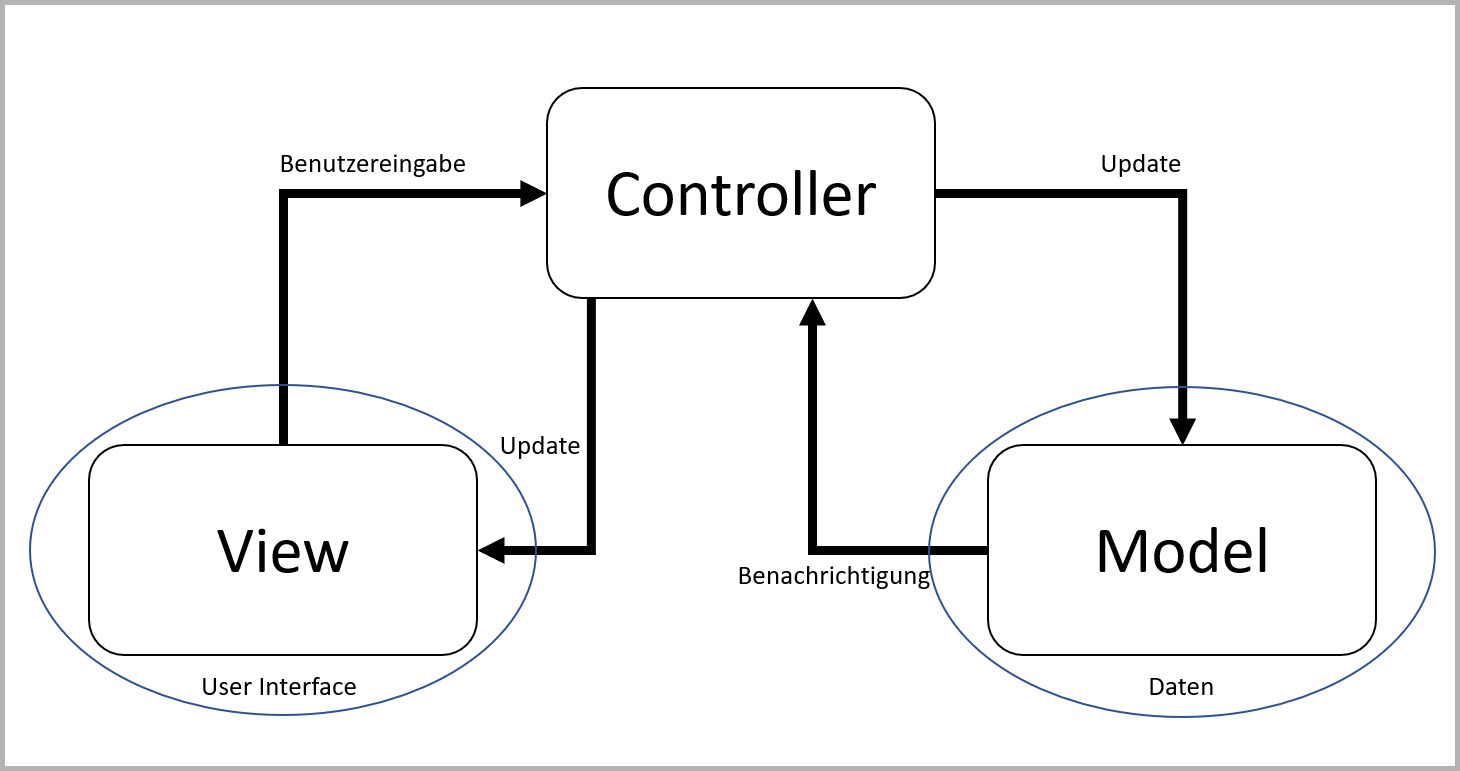
\includegraphics[width=0.75\linewidth]{images/rfoster_study/mvc}
	\caption[Übersicht des \textit{MVC-Patterns}]{Übersicht über die Komponenten des \textit{MVC-Patterns} und ihre Zusammenhänge}
	\label{fig:mvc}
\end{figure}
\subsubsection{MVVM}
\textit{\Gls{mvvm}} oder auch \textit{\Gls{mvvc}} ist ein \Gls{designpattern} mit dem eine Software in drei Teile geteilt wird \cite{mvvm_vue}. Jedoch wird bei \textit{MVVM} die Software in \textit{Model}, \textit{View} und \textit{ViewModel} aufgeteilt. 
Das \textit{Model} beinhaltet, wie im konventionellen \textit{\Gls{mvc}-Pattern}, alle wichtigen Daten und Funktionen. 
Die \textit{View} ist, wie beim \textit{MVC-Pattern}, der Teil der Software, mit dem der Benutzer interagiert. 
Das \textit{ViewModel} ist ein Bindeglied zwischen \textit{Model} und \textit{View} \cite{mvvm_vue}. Dabei stellt das \textit{ViewModel} der \textit{View} Funktionen zur Verfügung. Diese können auch Daten verändern bzw. mit Daten rechnen. Das Model kann über das \textit{ViewModel} auch mit der \textit{View} direkt interagieren. 
\textit{MVVM} sieht nicht vor, dass ein \textit{Controller} verwendet wird. Diese Funktion übernimmt zu einem gewissen Teil das \textit{ViewModel} bzw. auch die \textit{View} und das \textit{Model}.
\begin{figure}[H]
	\centering
	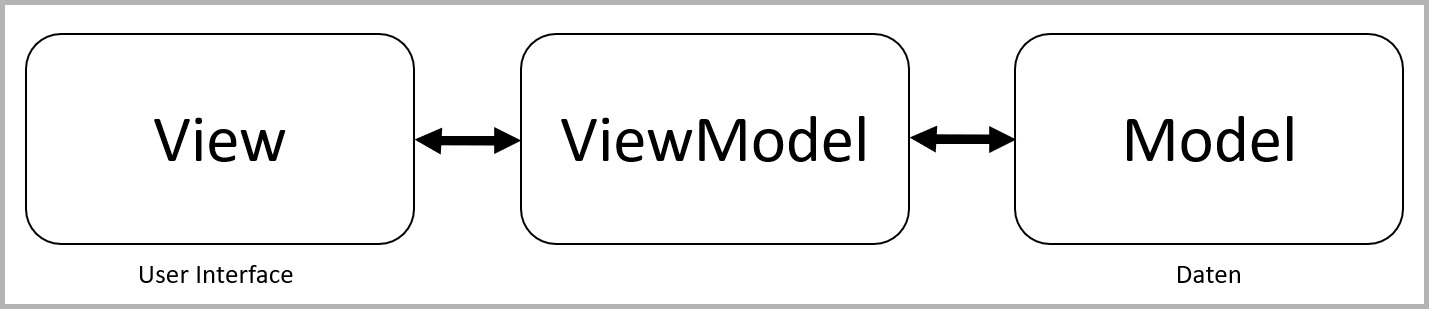
\includegraphics[width=0.8\linewidth]{images/rfoster_study/mvvm}
	\caption[Übersicht des \textit{MVVM-Patterns}]{Übersicht über die Komponenten des \textit{MVVM-Patterns} und ihre Zusammenhänge}
	\label{fig:mvvm}
\end{figure}
\subsubsection{Vergleich}
Diese zwei \Gls{designpattern} sind zwar sehr ähnlich, jedoch gibt es wichtige Unterschiede zwischen ihnen.\\\\
\textit{\Gls{mvc}} ist ein Entwurfsmuster, welches auf einem niedrigen Level überall im Einsatz ist - z.B. bei Tastatureingaben \cite{mvc}. Dieses Entwurfsmuster ist zwar schon lange verfügbar, jedoch kann es bei \textit{Webapplikationen} zu Problemen führen.\\
Bei der Entwicklung einer \textit{Webapplikation} ist es nicht einfach, das \textit{Model} von dem \textit{Controller} zu trennen.\\
\textit{\Gls{mvvm}} auf der anderen Seite zielt explizit auf \textit{HTML5} ab \cite{mvvm_vue}. Somit ist es bei webbasierten Applikationen zu bevorzugen.
\newpage
\subsection{Umsetzungsmöglichkeiten}
Dieser Teil des Projekts wird mittels \textit{\Gls{js}} umgesetzt. Hierbei kommen unterschiedliche \textit{\Gls{js}-\Gls{framework}s} in Frage. Hier werden die verbreitetsten \textit{JavaScript-Frameworks} vorgestellt und dann verglichen. \textit{\Gls{angular}} wird nicht in Betrachtung gezogen, da dies ein \textit{\Gls{framework}} für professionelle Projekte und demnach nicht für vergleichsweise kleine Projekte verwendbar ist, wegen dem Aufwand das \textit{Framework} zu erlernen \cite{angular_ex}.
\subsubsection{VueJS}
\textit{\Gls{vue}} ist ein progressives \textit{JavaScript-Framework}. Dies bedeutet, dass \textit{VueJS} in bereits bestehende Webseiten bzw. in webbasierte Software implementiert werden kann.\\
\textit{VueJS} kann aber auch von Anfang an verwendet werden, wobei man hier mit den Bibliotheken von \textit{VueJS} skalieren kann \cite{vuedoc}. \textit{VueJS} kann Teile einer Webseite in Komponenten aufteilen, um diese mehrmals zu verwenden, falls dies notwendig ist. Jeder dieser Komponenten besitzt seine eigene \textit{\Gls{html}}-, \textit{\Gls{css}}- und \textit{\Gls{js}} Datei, die gebraucht werden, um diese Komponente zu rendern.\\
Um einzelnen Elementen \textit{VueJS}-Funktionalität zu geben, kann auf diese Elemente folgender \textit{Code} angewendet werden \cite{vuedoc}:
\begin{code}{html}
	<!DOCTYPE html>
	<html lang="de">
		<head>
			<meta charset="UTF-8">
			<meta name="viewport" content="width=device-width, initial-scale=1.0">
			<title>Kurzes VueJS-Beispiel</title>
		</head>
		<body>
			<h1>Überschrift</h1>
			<div id="app">
				<!-- Der Text, welcher weiter unten Definiert wird, wird hier eingefügt -->
				<!-- Ändert sich die Variable, dann ändert sich auch der Text auf der Webseite -->
				<p> {{ text }} </p>
			</div>
			<script src="https://unpkg.com/vue"></script>
			<script>
				const app = new Vue({
					el: '#app',
					data: {
						text: 'Hier steht Text!'
					}
				})
			</script>
		</body>
	</html>
\end{code}
\captionof{listing}[\textit{VueJS} Beispiel]{Beispiel für \textit{VueJS} Webseite}~\\
\subsubsection{React}
\textit{\Gls{react}} ist eine \textit{\Gls{js}}-Bibliothek, mit der man Benutzeroberflächen entwickeln kann \cite{reactdoc}. \textit{React} hat, wie \textit{\Gls{vue}}, Komponenten. Dies bedeutet, dass man einzelne Elemente mehrfach verwenden kann, falls man dies benötigt.\\
\textit{React} wurde von Facebook entwickelt und wurde 2013 als \textit{\Gls{opensource}}-Lösung veröffentlicht.\\
Folgender \textit{Code} beschreibt eine Beispiel-\textit{React}-Webseite \cite{reactdoc}:
\begin{code}{html}
	<!DOCTYPE html>
	<html lang="de">
		<head>
			<meta charset="UTF-8">
			<meta name="viewport" content="width=device-width, initial-scale=1.0">
			<title>Kurzes React-Beispiel</title>
		</head>
		<body>
			<h1>Überschrift</h1>
			<div id="likebuttoncontainer"></div>
			
			<!-- Load React. -->
			<!-- Note: when deploying, replace "development.js" with "production.min.js". -->
			<script src="https://unpkg.com/react@17/umd/react.development.js" crossorigin></script>
			<script src="https://unpkg.com/react-dom@17/umd/react-dom.development.js" crossorigin></script>
			<!-- Load our React component. -->
			<script src="likebutton.js"></script>
		</body>
	</html>
\end{code}
\captionof{listing}[\textit{React}-Webseite Beispiel]{Beispiel für \textit{React} Webseite}~\\
\newpage
In der letzten Zeile des \textit{body-Tags}, wird auf \textit{likebutton.js} referenziert. Dies ist eine Komponente und muss noch erstellt werden \cite{reactdoc}:
\begin{code}{js}
	'use strict';
	
	const e = React.createElement;
	
	class LikeButton extends React.Component {
		constructor(props) {
			super(props);
			this.state = { liked: false };
		}
		
		render() {
			if (this.state.liked) {
				return 'You liked this.';
			}
			
			return e(
			'button',
			{ onClick: () => this.setState({ liked: true }) },
			'Like'
			);
		}
	}
	
	const domContainer = document.querySelector('#likebuttoncontainer');
	ReactDOM.render(e(LikeButton), domContainer);
\end{code}
\captionof{listing}[\textit{React}-Komponente Beispiel]{Beispiel für eine \textit{React}-Komponente}
\newpage
\subsubsection{Ohne Framework}
Die Schnittstelle zwischen \textit{\Gls{backend}} und \textit{\Gls{frontend}} kann auch ohne ein \textit{\Gls{framework}} umgesetzt werden. Dies ist bei kleinen und leichten Applikationen von Vorteil, da keine umständlichen \textit{\Gls{js}-\Gls{framework}s} aufgesetzt und richtig implementiert werden müssen. Ohne \textit{Framework} implementiert man eine \textit{\Gls{js}}-Datei in eine Webseite, um die gewünschte Funktionalität einzufügen. Mit folgendem \textit{Code} kann eine Implementierung einer \textit{JavaScript}-Datei umgesetzt werden:
\begin{code}{html}
	<!DOCTYPE html>
	<html lang="de">
		<head>
			<meta charset="UTF-8">
			<meta name="viewport" content="width=device-width, initial-scale=1.0">
			<title>Kurzes Plain-Beispiel</title>
		</head>
		<body>
			<div id="inhalt">
				<h1>Überschrift</h1>
			</div>
			<!-- Die Implementierung der JavaScript-Datei -->
			<script src="javascript.js"></script>
		</body>
	</html>
\end{code}
\captionof{listing}[Ohne \textit{Framework} Beispiel]{Beispiel für Webseite ohne \textit{Framework}}~\\
Es kann auch direkt in eine \textit{\Gls{html}}-Datei \textit{\Gls{js}} in ein \textit{<script></script>} geschrieben werden.
\newpage
\subsubsection{Vergleich}

Verglichen werden diese unterschiedlichen Umsetzungsmöglichkeiten an Gestaltung, Entwicklungszeit, Performanz und \Gls{loc}.\\
Die Webseite, die für den Vergleich umgesetzt werden soll, wird mit den unterschiedlichen Umsetzungsmöglichkeiten umgesetzt.\\
\begin{figure}[H]
	\centering
	
\includegraphics[width=0.8\linewidth]{images/rfoster_study/example_page}
	\caption[Die Beispielwebseite]{Die Beispielwebseite, die mit den Umsetzungsmöglichkeiten umgesetzt werden soll.}
	\label{fig:example}
\end{figure}
Folgende Tabelle zeigt die unterschiedlichen Werte bei der Umsetzung der Beispielwebseite:
\begin{table}
	\captionof{table}[Vergleich \textit{JavaScript-Frameworks}]{Vergleich von \textit{\Gls{js}-\Gls{framework}s}}\label{tab:vergleich}
	\centering
	\refstepcounter{table}
	\label{center}
	\begin{tabular}{l|c|c|c|c}
		Kriterium        & Maximale Punkte & \textit{VueJS} & \textit{React} & Ohne \textit{Framework}  \\\hline
		Gestaltung           & -                        &            \checkmark               &             \checkmark              &          \checkmark                           \\
		Entwicklungszeit & 9                         &             8              &               6            &               9                      \\
		Performanz       & 9                         &             7              &               4            &                 9                    \\
		\textit{\Gls{loc}}              & 9                         &             9              &               8            &                   2                  \\
		Gesamtpunkte     & 27                         &              24             &               18            &                20                    
	\end{tabular}
\end{table}
\textbf{Kriterien:}\\\\
\textbf{Gestaltung}\\
Die Gestaltung fällt in die Wertung, da hier angegeben wird, ob die Beispiel-Webseite so umgesetzt werden kann oder ob die Umsetzung in dieser Gestaltung nicht möglich ist.\\\\
\newpage
\textbf{Entwicklungszeit}\\
\textit{\Gls{vue}}: 40min\\
\textit{\Gls{react}}: 55min\\
\textit{Ohne \Gls{framework}}: 20min\\
Die Entwicklungszeit zwischen den zwei \textit{\Gls{framework}s} ist sehr ähnlich. Jedoch ist zu beachten, dass bei dem \textit{VueJS-Framework} bereits mit Komponenten gearbeitet worden ist und dadurch die Entwicklungszeit höher ist als notwendig. Ohne \textit{Framework} war die Entwicklungszeit am kürzesten, da nichts installiert, importiert oder aufgesetzt werden musste.\\\\
\textbf{Performanz}\\
\textit{\Gls{vue}:} 112ms\\
\textit{\Gls{react}}: 175ms\\
\textit{Ohne \Gls{framework}}: 21ms\\
\textit{Ohne Framework} ist die Performanz sehr gut, da im Hintergrund keine \textit{Frameworks} geladen werden müssen. Das \Gls{js} wird direkt ausgeführt. Bei \textit{VueJS} und \textit{React} werden viele Bibliotheken im Hintergrund geladen, wodurch die Performanz sinkt. Obwohl Komponenten bei der Umsetzung mittels \textit{VueJS} verwendet worden sind, ist \textit{VueJS} performanter als \textit{React}.\\\\
\textit{\textbf{Lines of Code}}\\
Die beiden \textit{Frameworks} haben besonders gut abgeschnitten, da für die Umsetzung mit \textit{VueJS} nur wenige \textit{Codezeilen} geschrieben werden mussten. Durch die Funktionalität von \textit{VueJS} können viele \textit{Codezeilen} eingespart werden. \textit{React} ist in dem Aspekt für das Projekt geeignet, da auch sehr wenige \textit{Codezeilen} geschrieben werden mussten. Jedoch musste bei \textit{React} deutlich mehr entwickelt werden, wodurch es nicht die vollen Punkte erreicht.
Ohne \textit{\Gls{framework}} konnten weniger Punkte erreicht werden, da die Umsetzung im Vergleich nicht nur unübersichtlicher und komplizierter ist, sondern auch damit zu rechnen ist, dass die Umsetzung bei größeren Beispielen zu großen Problemen führen kann.
\newpage
\subsection{Aufbereitung der Daten}
Die Daten, welche von der \textit{REST}-Schnittstelle gelesen werden, sind im \textit{\Gls{json}}-Format. Dies wird genauer im \autoref{sec:json} erklärt. Um die Daten von der \textit{REST}-Schnittstelle zu bekommen, wird \textit{\Gls{axios}} verwendet. Mit dieser Bibliothek kann eine \textit{\Gls{http}}-Anfrage gesendet und damit die Daten von der \textit{REST}-Schnittstelle ausgelesen werden. Im folgenden \textit{Code} wird eine Beispiel-Anfrage gesendet:
\begin{code}{html}
	<html>
		<head>
			<!-- Import von Axios -->
			<script src="https://unpkg.com/axios/dist/axios.min.js"></script>
			<meta charset="UTF-8">
			<title>Axios-Anfrage</title>
		</head>
		<body>
			<script>
				// Anfrage an den Server um die Daten zu bekommen
				axios.get("http://localhost:3000/data").then(response => {
					//Die Daten, die zurückkommen werden in der Konsole ausgegeben
					console.log(response.data);
				})
			</script>
		</body>
	</html>
\end{code}
\captionof{listing}[\textit{HTTP}-Anfrage mittels \textit{Axios}]{Umsetzung einer \textit{HTTP}-Anfrage mittels \textit{Axios}}~\\
Die Daten, welche von der Anfrage zurückkommen, können dann verwendet werden, um \textit{\Gls{html}}-Elemente zu erstellen oder zu verändern, um das \textit{\Gls{frontend}} dynamisch mit den Daten zu füllen.\\Nachdem nicht alle Daten immer benötigt werden, kann bei den Anfragen die Endung verändert werden, um spezifische Daten abzufragen. Dies muss natürlich von der \textit{REST}-Schnittstelle unterstützt werden. Eine Beispielanfrage für solch eine spezifische Anfrage ist wie folgt:
\begin{code}{js}
	// Hier werden z.B.: die Daten von dem Benutzer 1234 abgefragt.
	axios.get("http://localhost:3000/user/1234/infos").then(response => {
		//Die Daten, die zurückkommen werden in der Konsole ausgegeben
		console.log(response.data);
	})
\end{code}
\captionof{listing}[\textit{Axios} Anfrage mit genauem Pfad]{Umsetzung einer \textit{Axios} Anfrage unter Verwendung eines genauen Pfades}~\\
Die praktische Durchführung ist, wie bereits im vorherigen Kapitel besprochen, bei den Umsetzungsmöglichkeiten unterschiedlich.
\subsection{Fazit}
\label{sec:rfoster_fazit}
Nach dieser Arbeit ist die Entscheidung für eine Umsetzungsmöglichkeit einfach. \textit{\Gls{mvvm}} ist genau auf webbasierte Anwendungen zugeschnitten und bei \textit{\Gls{vue}} kann durch die vordefinierten Komponenten viel Zeit und Arbeit gespart werden. \textit{VueJS} hat im Vergleich zu \textit{\Gls{react}} den Vorteil, dass hier bereits mehr Erfahrung in der Umsetzung besteht, woraus folgt, dass \textit{VueJS} die effizienteste Variante für die Umsetzung ist.